\documentclass{beamer}

\usepackage{ctex}

\usetheme{Berkeley}
% \usetheme{Berkeley}

\if false 
	各种各样的主题
	http://www.ctan.org/tex-archive/macros/latex/contrib/beamer/doc/
	Antibes Bergen Berkeley Berlin
	Boadilla Copenhagen Darmstadt Dresden
	Frankfurt Goettingen Hannover Ilmenau
	Juanlespins Madrid Malmoe Marburg
	Montpellier Paloalto Pittsburgh Rochester
	Singapore
	
	颜色主题 \usecolortheme{default}
	color theme: albatross crane beetle dove fly seagull wolverine beaver
	inner color: lily orchid rose
	outter color: whale seahorse dolphin
\fi

\title[short title]{long title}
\subtitle[short subtitle]{long subtitle}
\author[short name]{long name}
\date[short date]{long date}
\institute[short name]{long name}
\titlegraphic{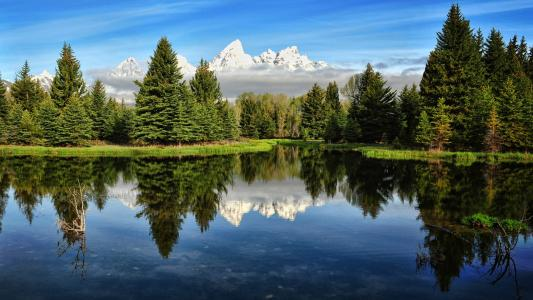
\includegraphics[width=0.17\textwidth]{image.jpg}}

\begin{document}
	
	% 标题页帧
	\frame{\titlepage}

	\begin{frame}[label = outline]
		\frametitle{Outline}
		% \tableofcontents[part=1,pausesections]
		\tableofcontents
	\end{frame}

	% 普通帧
	\begin{frame}[c] % c表示对齐方式
		\frametitle{frame title}
		The is the content
		\hyperlink{outline}{\beamergotobutton{sadad}}
	\end{frame}

	% 空白帧
	\begin{frame}[plain]
		空白帧是没有标题的
	\end{frame}

	% 节和小节
	
	\section{section name}
	\subsection{subsection name}
	\subsubsection{sub-subsection name}
	\section*{section name}	% * 不进入目录
	
	
	% 列表
	\begin{frame}[c]
		\frametitle{无序列表}
		\begin{itemize}
			\item The first item
			\item The second item
			\item The third item
			\item The fourth item
		\end{itemize}
	\end{frame}

	\begin{frame}[c]
		\frametitle{有序列表}
		\begin{enumerate}
			\item The first item
			\item The second item
			\item The third item
			\item The fourth item
		\end{enumerate}
	\end{frame}

	\begin{frame}[c]
		\frametitle{描述列表}
		\begin{description}
			\item[First Item] Description of first item
			\item[Second Item] Description of second item
			\item[Third Item] Description of third item
			\item[Forth Item] Description of forth item
		\end{description}
	\end{frame}

	\begin{frame}[c]
		\frametitle{文本命令}
		\emph{Sample Text}
		
		\textbf{Sample Text}
		
		\textit{Sample Text}
		
		\textsl{Sample Text}
		
		\alert{Sample Text}
		
		\textrm{Sample Text}
		
		\textsf{Sample Text}
		
		\textcolor{green}{Sample Text}
		
		\structure{Sample Text}
	\end{frame}

	\begin{frame}[c] 
		\frametitle{字体设置}
		字体主题:\textbackslash usefonttheme[onlymath]{serif}
		
		字体大小:\textbackslash documentclass[11pt]{beamer},可选项为 10-11-12pt
		
		字体族 :\textbackslash usepackage{helvet},可选项为serif avant bookman chancery charter
		euler helvet mathtime mathptm mathptmx
		newcent palatino pifont utopia
	\end{frame}


	\begin{frame}[c] 	
		\frametitle{分栏}
		\begin{columns}
			\column{.5\textwidth}
			First column text and/or code
			\column{.5\textwidth}
			Second column text and/or code
		\end{columns}
	\end{frame}


	\begin{frame}[c] 	
		\frametitle{内部环境}
		block 普通环境
		
		theorem 定理环境
		
		lemma 引理环境
		
		proof 证明环境
		
		corollary 推论环境
		
		example 示例环境
		
		alertblock 警示环境
	\end{frame}

	\begin{frame}[c] 	
		\frametitle{表格}
		\begin{table}[tb]
			\centering
			\caption{Caption here\label{tab:tablename}}
			\begin{tabular}{l|cc} \hline
				\textbf{column 1} & \textbf{column 2} & \textbf{column 3} \\ \hline
				Hello & Beamer & NAN \\ \hline
				$\alpha+\beta$ & $\gamma+\eta$ & 34\% \\ \hline
			\end{tabular}
		\end{table}
	\end{frame}

	\begin{frame}[c] 	
		\frametitle{插图}
		\begin{figure}[tb]
			\centering
			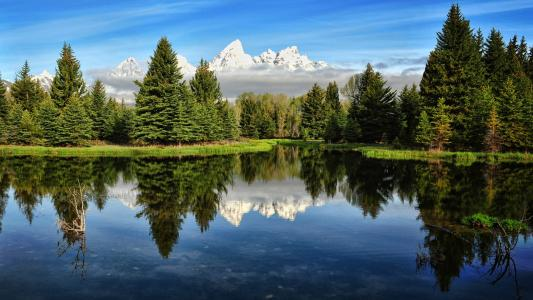
\includegraphics[width=0.9\textwidth]{image.jpg}
			\caption{Caption here\label{fig:figure1}}
		\end{figure}
	\end{frame}


	\begin{frame}[c]
		\frametitle{数学证明}
		\framesubtitle{证明的内容}
		\begin{theorem}
			定理	
		\end{theorem}
		\begin{proof}
			证明\qedhere
		\end{proof}
	\end{frame}

\end{document}